\documentclass{resume}
  \usepackage{graphicx}
  \usepackage{tabu}
  \usepackage{tabularx}
  \usepackage{multirow}
  \usepackage{progressbar}
  \usepackage{zh_CN-Adobefonts_external} % Simplified Chinese Support using external fonts (./fonts/zh_CN-Adobe/)
  %\usepackage{zh_CN-Adobefonts_internal} % Simplified Chinese Support using system fonts
  \usepackage{tikz}
  \usepackage{linespacing_fix} % disable extra space before next section
  \usepackage{cite}
  \usepackage{geometry}
  \geometry{a4paper,left=1.6cm,right=1.6cm,top=1cm,bottom=1cm}
  \begin{document}
  \pagenumbering{gobble} % suppress displaying page number
  % \name{张景涛}
  
  % \basicInfo{
  %   \email{sy1906605@buaa.edu.cn} \textperiodcentered\ 
  %   \phone{(+86) 178-5416-0892} % \textperiodcentered\ 
  %   % \linkedin[billryan8]{https://www.linkedin.com/in/billryan8}
  %   }
   
  \begin{minipage}{0.7\textwidth}
    \Large{
      \begin{tabu}  { l }
        \scshape{张\ 景\ 涛} \\
        \email{sy1906605@buaa.edu.cn} \\
        \phone{(+86) 178-5416-0892} \\
      \end{tabu}
    }
  \end{minipage}
  \begin{minipage}{0.3\textwidth}
    \raggedleft
    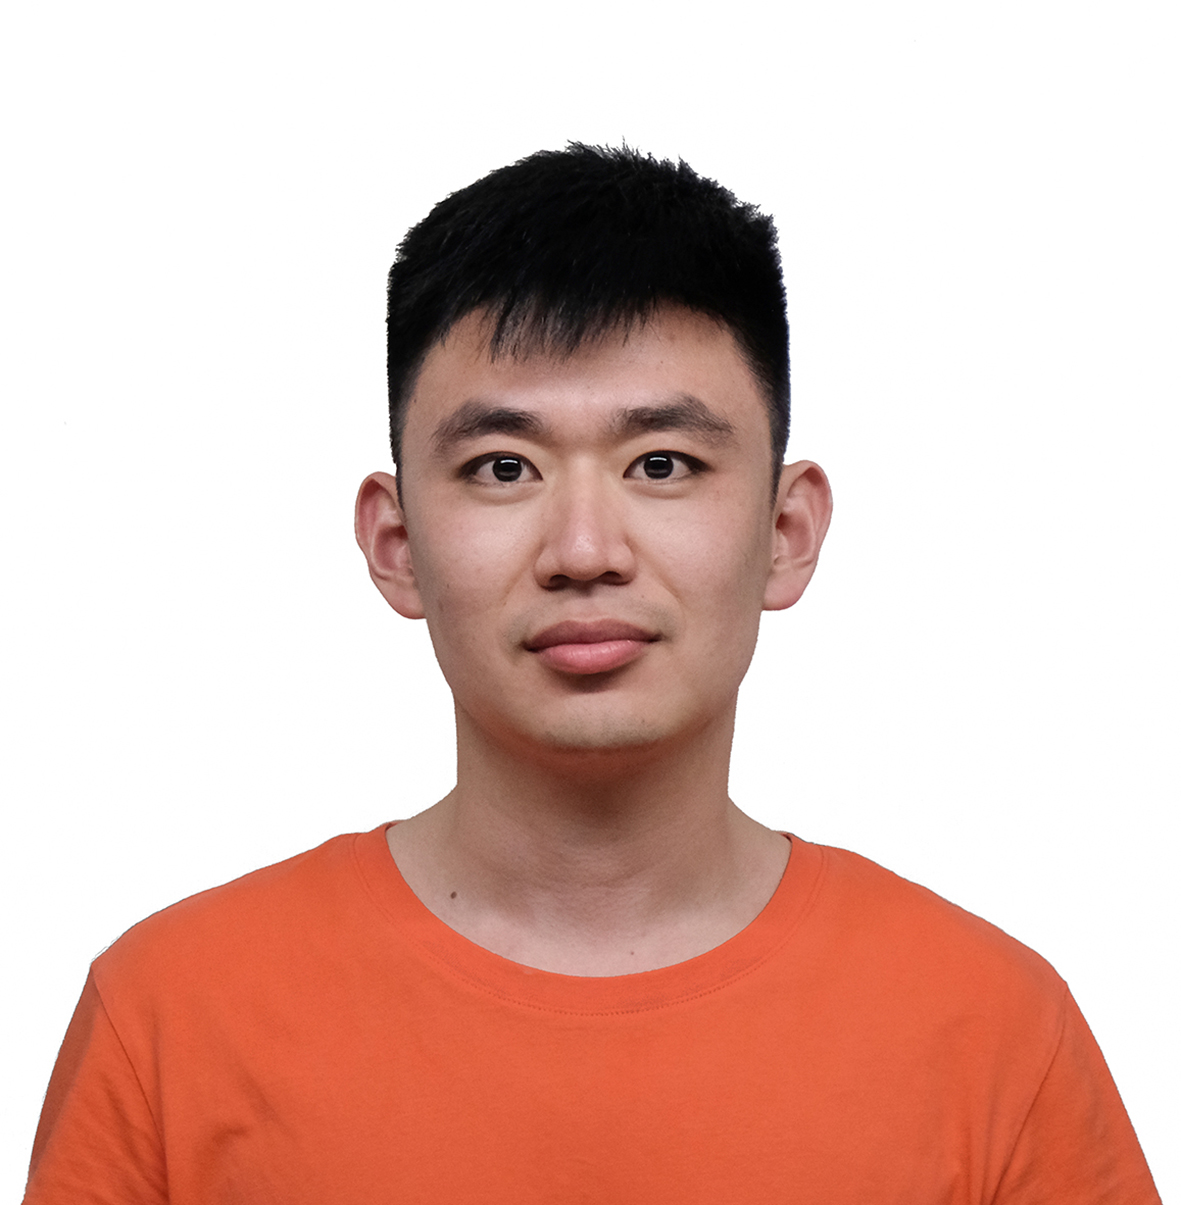
\includegraphics[height=30mm]{avatar}
  \end{minipage}
  
  \section{\faGraduationCap\ 教育背景}
  \datedsubsection{\textbf{北京航空航天大学}\ 北京}{2019.09 - 至今}
  \textit{在读硕士研究生}\ 计算机科学与技术专业\ 保研入学\ 预计2022.01毕业
  \datedsubsection{\textbf{山东大学}\ 济南, 青岛}{2015.09 - 2019.06}
  \textit{学士}\ 计算机科学与技术专业\ \ GPA: 4.68 / 5.0 (专业前2\%) \\
  荣誉: 国家奖学金(2017\&2018)、校级优秀学生干部(2016\&2017) \\
  奖项: 国际硬件设计竞赛三等奖、山东省大学生软件设计大赛一等奖、数学建模竞赛山东赛区二等奖
  
  \section{\faUsers\ 实习/项目经历}
  
  % \datedsubsection{\textbf{大规模轨迹表示与规律挖掘}}{2020.09 - 2021.11}
  % \role{编码器\ 表示学习}{研究生课题}
  % \begin{itemize}[topsep = 0 pt, partopsep = 0pt]
  %   \item 大规模的轨迹距离计算,利用编码器将轨迹序列编码成特征向量,将传统轨迹距离计算算法的时间复杂度降低到常数级别
  %   \item 时空一致性下的伴随,重复轨迹规律挖掘算法,探索中...
  % \end{itemize}
  
  \datedsubsection{\textbf{时代复兴\ 函数计算框架建设}}{2020.04 - 2020.09}
  \role{时代复兴\ 基础设施}{实习生}
  % \begin{onehalfspacing}
    参与函数计算框架的建设和维护工作。在熟悉kubernetes集群的基础上,深入了解改造了Fission函数计算框架,并在公司内部进行了推广。主要有如下两方面贡献:
  \begin{itemize}[topsep = 0 pt, partopsep = 0pt]
    \item 简化开发者编写部署函数的流程。通过提供函数创建模板、本地测试环境以及自动化部署脚本,让即使不熟悉kubernetes的开发人员,经过简单的培训,也能编写部署自己的服务。
    \item 丰富函数计算框架的功能。包括改进日志查看和投递功能、添加了函数的层级配置功能和数据流的可视化组件等,方便了用户的调试,简化了从测试环境向生产环境迁移函数的流程,并可以直观的看到整个项目的数据流动。
  \end{itemize}
    相关工作可参考\href{https://github.com/jingtaozhang18/fission}{Fission}和\href{https://github.com/jingtaozhang18/fission-template}{Fission Template}项目以及\href{https://jingtao.fun/%E6%BA%90%E7%A0%81-Fission%E5%8A%9F%E8%83%BD%E6%8B%93%E5%B1%95/}{改造总结文档} (已获得时代复兴的公开允许)。
  % \end{onehalfspacing}
  
  \datedsubsection{\textbf{字节跳动\ 质量保障平台建设}}{2019.03 - 2019.09}
  \role{字节跳动\ 头条研发}{实习生}
  % \begin{onehalfspacing}
  \begin{itemize}[topsep = 0 pt, partopsep = 0pt]
    \item 参与监控报警平台的维护工作,包括日志流(>1Mil/s)的实时处理和数据指标的定时查询。日志在消息队列中流动,经过计算引擎的处理后,写入ES、Metrics和Druid三种监控存储引擎中,并通过定时查询的方式得到监控数据的指标。
    \item 参与自动化内测系统的搭建工作,包括内测用户池的维护,内测用户的画像构建、奖励机制以及内测效果的评估等。在其中负责了自动化补充内测用户池的功能和内测效果的计算、展示模块等。
  \end{itemize}
  % \end{onehalfspacing}
  
  % \datedsubsection{\textbf{南京韧臻\ 在线考试平台建设}}{2018.07 - 2018.11}
  % \role{南京韧臻\ 开发组}{实习生}
  % % \begin{onehalfspacing}
  % \begin{itemize}[topsep = 0 pt, partopsep = 0pt]
  %   \item 在Spring MVC框架的基础上集成了异地两系统间的Mysql数据库的定时同步功能。
  %   \item 开发了考场机位容量测试组件,通过模拟考试过程中的流量,测试一个考场同时最多能容纳多少人考试。
  % \end{itemize}
  % % \end{onehalfspacing}

  \datedsubsection{\textbf{小型电影推荐系统}}{2018.03 - 2018.06}
  \role{山东大学\ 课程设计}{独立完成}
  % \begin{onehalfspacing}
  \begin{itemize}[topsep = 0 pt, partopsep = 0pt]
    \item 可以应对不同用户不同打分偏好的,基于协同过滤思想的小型电影推荐系统。
    \item 该系统基于Spark大数据框架,使用Scala编程语言实现。
  \end{itemize}
  % \end{onehalfspacing}

  \datedsubsection{\textbf{“智慧山大”便捷校园服务系统}}{2016.06 - 2017.10}
  \role{山东大学\ 齐鲁软件大赛}{队长}
  % \begin{onehalfspacing}
  \begin{itemize}[topsep = 0 pt, partopsep = 0pt]
    \item 该项目是一个依托Laravel的PHP框架,采用网页的形式,为学生生活提供查询,报修,论坛,自动选课,个人网盘,提醒重要网站的新通知等服务的系统。
    \item 在项目中,为系统编写了与山大官网对接的API(包括学生身份认证,重要网站自动爬虫对比等),创建维护数据库系统,组装云盘、论坛模块。并在云服务器上搭建了整个系统,并进行了测试。
  \end{itemize}
  % \end{onehalfspacing}
  
  % Reference Test
  %\datedsubsection{\textbf{Paper Title\cite{zaharia2012resilient}}}{May. 2015}
  %An xxx optimized for xxx\cite{verma2015large}
  %\begin{itemize}
  %  \item main contribution
  %\end{itemize}
  
  \section{\faCogs\ 技能}
  % increase linespacing [parsep=0.5ex]
  \begin{itemize}[parsep=0.5ex]
    \item 编程语言: C++ Python Go
    \item 开发工具: Linux Git Docker
    \item 英语: CET6
  \end{itemize}
  
  % \section{\faHeartO\ 获奖情况}
  % \datedline{国家奖学金}{2017.10 \& 2018.10}
  % \datedline{校级优秀学生干部}{2016.10 \& 2017.10}
  % \datedline{国际硬件设计竞赛三等奖}{2017}
  % \datedline{第十五届山东省大学生软件设计大赛一等奖}{2017}
  % \datedline{全国大学生数学建模竞赛\ 山东赛区二等奖}{2017}
  
  % \section{\faInfo\ 其他}
  % % increase linespacing [parsep=0.5ex]
  % \begin{itemize}[parsep=0.5ex]
  %   \item 技术博客: \href{https://jingtao.fun}{https://jingtao.fun}
  %   \item GitHub: \href{https://github.com/jingtaozhang18}{https://github.com/jingtaozhang18}
  %   \item 语言: 英语 - CET6
  % \end{itemize}
  
  %% Reference
  %\newpage
  %\bibliographystyle{IEEETran}
  %\bibliography{mycite}
  \end{document}
